% siminos/spatiotemp/chapter/models.tex
% $Author: predrag $ $Date: 2021-12-24 01:25:20 -0500 (Fri, 24 Dec 2021) $

\section{Gaussian model}
\label{sect:GaussianModel}
\renewcommand\speriod[1]{{\ensuremath{\ell_{#1}}}}  %continuous spatial period
\renewcommand\period[1]{{\ensuremath{\ell_{#1}}}}  %continuous time period
\renewcommand{\ssp}{\ensuremath{\phi}}             % lattice site field
\renewcommand{\Ssym}[1]{{\ensuremath{m_{#1}}}}    % Boris


\begin{description}
\item[2019-11-04 Predrag]
Ivashkevich, Izmailian and Hu\rf{IvIzHu02} {\em Kronecker's double series
and exact asymptotic expansions for free models of statistical mechanics
on torus}:

{\em Gaussian model} is a boson analog of Ising model. Consider square
lattice of size $N\times M$ wrapped on a torus. To each site
$(m,n)$ of the lattice we assign a continuous variable $\field_{mn}$.
The Hamiltonian of the model is
\begin{equation}
H(\field)=-J\sum_{n=0}^{N-1}\sum_{m=0}^{M-1}
\left(\field_{mn}\,\field_{m+1,n}
      -2\field^2_{mn}
      +\field_{mn}\,\field_{m,n+1}
\right)
\,,
\label{BosonHamiltonian}
\end{equation}
with the partition function
%
$$Z(J)=\int_{\reals^{MN}} e^{-H(\field)}~{\rm d}\sigma(\field)$$
%
If the measure ${\rm d}\sigma(\field)$ in the phase space ${\reals^{MN}}$ is
Gaussian
%
$$ {\rm d}\sigma_{\rm
Gauss}(\field)=\pi^{-MN/2}\prod_{n=0}^{N-1}\prod_{m=0}^{M-1}
e^{-\field^2_{mn}}~ {\rm d}\field_{mn} $$
%
the integration can be done explicitly and the partition function
of the free boson model can be written in terms of the partition
function with twisted boundary conditions % Eq.(\ref{Zab})
\begin{equation}
Z_{\alpha,\beta}(\mu)=\prod_{n=0}^{N-1} 2\left| \textstyle{~\!{\rm
sh}\left[M\omega_\mu\!\left(\frac{\pi(n+\alpha)}{N}\right)+i\pi\beta
\right] }\right| \label{Zab1}
\end{equation}
and
parameterization $J^{-1}=4\,{\rm ch}^2\,\mu$ as
\begin{equation}
Z_{\rm Gauss}(\mu)=\left(\sqrt{2}\;{\rm
ch}\,\mu\right)^{MN}~\Big[\;Z_{0,0}(\mu)\;\Big]^{-1}
\label{ZBoson}
\end{equation}
where
\beq
Z^2_{0,0}(\mu)=
\prod_{n=0}^{N-1}\prod_{m=0}^{M-1}4\left[\textstyle{
\;\sin^2\left(\frac{\pi n }{N}\right)+
\sin^2\left(\frac{\pi m}{M}\right)+2\,{\rm sh}^2\mu
\;}\right]
\,.
\ee{Zab00}
This model exhibit phase transition at the point $\mu_c=0$ where
the partition function is divergent. This is due to the presence
of so-called zero mode, i.e. due to the symmetry transformation
$\field_{mn}\to \field_{mn}+{\rm const}$, which leave the Hamiltonian
(\ref{BosonHamiltonian}) invariant. Correlation functions of
disorder operator in this model have been studied by Sato, Miwa
and Jimbo.
    % \cite{SatoMiwaJimbo}.
    % Sato,~M., Miwa,~T. and Jimbo,~M.: {\it Holonomic Quantum Fields V},
    % Publ. RIMS, Kyoto Univ. {\bf 16}, 531 (1980).

The reason why this model is often considered as boson analog of
the Ising model is that one can choose another measure in the
phase space, which makes this model equivalent to the Ising model
considered above
%\begin{equation}
$$ {\rm d}\sigma_{\rm
Ising}(\field)=2^{-MN}\prod_{n=0}^{N-1}\prod_{m=0}^{M-1}
\big[\,\delta(\field_{mn}-1)+\delta(\field_{mn}+1)\,\big]~ {\rm
d}\field_{mn} $$
%\end{equation}
where $\delta$'s are Dirac $\delta$-functions. With such a
definition the variables $\field_{mn}$ can actually take only two
values: $+1$ or $-1$, so that $\field^2_{mn}=1$. In this case
integration can be replaced by summation over discrete values of
$\field_{mn}=\pm 1$ and the Hamiltonian (\ref{BosonHamiltonian})
coincides with the Hamiltonian of the Ising model
(\ref{IsingHamiltonian}) up to a constant.

\item[2020-06-19 Predrag]

Connect to \refeq{ActionPC}?

Recheck {\bf [2019-09-25 PC]}
Levit and Smilansky?

\item[2020-06-19 Predrag]
P. A. P. Moran\rf{Moran73}
{\em A Gaussian Markovian Process on a Square Lattice}
%  DOI: 10.2307/3212495  https://www.jstor.org/stable/3212495
is a very good paper that does all the right stuff with the Gaussian
``model,'' and ends up with the complete elliptic integral of the first
kind \refeq{Cserti00(38)}.

\item[2020-06-19 Predrag]
% not relevant: https://doi.org/10.1103/PhysRevB.31.5954
% not relevant: http://www.icmp.lviv.ua/journal/zbirnyk.21/011/art11.pdf
% Tom Kennedy \HREF{https://www.math.arizona.edu/~tgk/541/chap4.pdf}
% {\em 4  Random walks}

Eduardo Fradkin\rf{Fradkin13} {\em Field Theories of Condensed Matter Physics},
discusses on p.~336
the quantum partition function of the dimer model which is given by the classical
partition function of a discrete Gaussian model in three Euclidean dimensions on
a cubic lattice. See also p.~332, 345 and 354. Not sure how to connect it to our work.

Shankar\rf{Shankar17} {\em Quantum Field Theory and Condensed Matter}
defines the Gaussian model in Eqs.~(13.2), (6.219);
sect~{\em 11.1 The renormalization group: first pass};

Marino\rf{Marino17} {\em Quantum Field Theory Approach to Condensed
Matter Physics}
(see {\em 5.2 Gaussian Functional Integrals}) does not seem to refer to
the Gaussian model.

Chaikin and Lubensky\rf{ChaLub95} {\em Principles of Condensed Matter Physics}
see {\em 5.3 Gaussian integrals},  {\em 5.8.3 Gaussian model}

\emph{Lattice 89: Proceedings of the 1989 Symposium on Lattice Field Theory}
edited by N. Cabbibo, E. Marinari, G. Parisi

\item[2020-09-06 Predrag]
Kadanoff\rf{Kadanoff00} on Gaussian model:  sect.~{\em 3.4 Lattice Green Function}
and many more.
The ``coefficients matrix'' $C$ in Kadanoff eq.~(3.9) is the inverse
of my `propagator' $\Delta$.

A lattice with one field $\ssp_n$ for each site, then we can define a
particularly simple and important problem by giving the coefficient
matrix
Kadanoff eq.~(3.12)
\beq
C   =
\left(\begin{array}{ccccccc}
 {1}& -{K}& 0 & 0 &\dots &0& -{K}\\
 -{K}&  {1}& -{K}& 0 &\dots &0&0 \\
0 & -{K}&  {1}& -{K}&\dots &0 & 0 \\
\vdots & \vdots &\vdots & \vdots & \ddots &\vdots &\vdots\\
0 & 0 & \dots &\dots &\dots  & {1}& -{K}\\
 -{K}& 0 & \dots &  \dots &\dots& -{K}&  {1}
        \end{array} \right)
\,.
\ee{Kadanoff(3.12)}
The on-site interaction normalizes the Gaussian variables, for $K=0$
one gets the usual multi\dmn\ Gaussian.
$-K$ is the nearest neighbor coupling strength,
related to our case be $-{s}\to1$, off-diagonal $1\to-K$, so
the conversion is $s=-1/K$ (I believe).

Fourier transform of the $d$\dmn\ Green's function Kadanoff eq.~(3.19)
\beq
G(q)   = \frac{1}
         {1 - 2K\sum_{j=1}^d \cos(2\pi k_j/\speriod{j})}
         \,,\qquad
         q_j=
\ee{Kadanoff(3.19)}

Compare with \refeq{Harshaw16a} and our Fourier-transformed field for
$k$th discrete $d$\dmn\ Fourier component on
$\speriod{1},\speriod{2},\cdots,\speriod{d}$ torus,
no tilt,
\beq
\hat{\ssp}_k
= \frac{1}{d{s} - 2\sum_{j=1}^d \cos(2\pi k_j/\speriod{j})}\,\hat{\Ssym{}}_k
\,,
\ee{FourieTrField1}
where
\(
k=(k_1,k_2,\cdots,k_d)\,,
\)
so
\beq
K  = \frac{1}
         {d{s}}
\,,
\ee{Kadanoff-us}

Kadanoff eq.~(4.38) shows that the $d$\dmn\ Gaussian model only makes
sense when $K$ is in the interval $[-1/2d,1/2d]$, \ie, if $|{s}|>2$. If
$|K|$ exceeds this limit (Kadanoff says ``dragons live here''), the
Gaussian integrals diverge at infinite q-values, and the whole problem
stops making sense. When there is any qualitative change in behavior of a
many particle system we say that it undergoes a phase transition. The
Gaussian model does so at the two points $K=\pm1/2d$.

I still have some (conceptual) sign problems, as Kadanoff shows that his
allowed values $K$ correspond to harmonic oscillator states. I would like
that to correspond to $|{s}|<2$. I also need to explain why \catlatt\ has
grammar, while Gaussian model has no restrictions... Still do not
understand why all our {\HillDet}s have an ${\mu}^2$ prefactor. Inconclusive.


\end{description}
\renewcommand\speriod[1]{{\ensuremath{L_{#1}}}}  %continuous spatial period
\renewcommand\period[1]{{\ensuremath{T_{#1}}}}  %continuous time period
\renewcommand{\ssp}{x}
\renewcommand{\Ssym}[1]{{\ensuremath{s_{#1}}}}  % ChaosBook


\section{Tight-binding Hamiltonians}
\label{sect:TightBind}
% moved from siminos/spatiotemp/chapter/QFTlatt.tex 2020-11-01

\begin{description}
  \item[2017-09-11 Predrag]
Economou\rf{Economou06} {\em {Green's Functions in Quantum Physics}}
\CBlibrary{Economou06}
contains a vast amount of useful information.
Lattice shows up in chap.~5 {\em Green's Functions
for tight-binding Hamiltonians}. Extracted text:
\end{description}

``[...] the Green's functions for the so-called tight-binding Hamiltonian
(TBH) are calculated. The TBH is of central importance for solid-state
physics because it is the simplest example of wave propagation in
periodic structures. It is also important for quantum physics in general
because it is rich in physical phenomena (e.g., negative effective mass,
creation of a bound state by a repulsive perturbation) and, at the same
time, simple in its mathematical treatment. Thus one can derive simple,
exact expressions for scattering cross sections and for bound and
resonance levels. The multiple scattering formalism is presented within
the framework of the TBH and applied to questions related to the behavior
of disordered systems (such as amorphous semiconductors).''

He studies the Green's functions associated with a class of periodic
Hamiltonians, i.e., Hamiltonians remaining invariant under a translation
by any vector on a regular $d$\dmn\ lattice.

He also considers the more general case where the lattice can be divided
into two interpenetrating sublattices such that each point of sublattice
1 is surrounded by points belonging to sublattice 2; the Hamiltonian
remains invariant under translation by vectors of sublattice 1 or
sublattice 2.

Periodic Hamiltonians are mathematically equivalent to a system of
coupled 1-d harmonic oscillators and, as a result, they describe (by
direct generalization to 3-d) the ionic motions in a crystalline solid.

In this approach one views the solids as being made up of atoms brought
together from an infinite relative distance. It is then natural (following the
usual practice for molecules) to try to express the unknown electronic wave
functions as linear combinations of atomic orbitals (LCAO).
The simplest version of this approach considers
only one atom per primitive crystal cell, only one atomic orbital per atom,
nearest-neighbor coupling only, and orthonormality of the atomic orbitals.
This oversimplified version of the LCAO is known as the tight-binding
model (TBM); the atomic orbital associated with the atom located at site $\ell$
is symbolized by
\beq
w(r-\ell) = \braket{{r}}{\ell}
\,.
\ee{Economou06(5.4)}
The matrix elements of the Hamiltonian within
this subspace are
\beq
H=\sum_\ell\ket{\ell}\epsilon_\ell\bra{\ell}
  + \sum_{\ell m}\ket{\ell}V_{\ell m}\bra{m}
\,.
\ee{Economou06(5.7)}
The diagonal matrix elements are denoted
by $\epsilon_\ell$ and the off-diagonal matrix elements by
$V_{\ell m}$ ($V_{\ell\ell} = 0$).
The periodicity of the Hamiltonian, i.e., its invariance under translations
by a lattice vector $\ell$, implies that
\beq
\epsilon_\ell=\epsilon_0
\ee{Economou06(5.6a)}
\beq
V_{\ell m}=V_{\ell-m}
\,.
\ee{Economou06(5.6b)}
For the sake of simplicity one assumes that
\beq
   V_{\ell m} = \left\{
     \begin{array}{ll}
         V & \mbox{if\ } \ell,m \mbox{ nearest neighbors}\\
         0 & \mbox{otherwise}
     \end{array}
             \right.
\,.
\ee{Economou06(5.9)}
There is only one quantity, $V$, which, following the usual practice in
the literature, can be taken as negative (for s-like orbitals $V$ is
indeed negative).
\beq
H
  =
\left(\begin{array}{ccccccc}
 \epsilon_0& V & 0 & 0 &\dots &0& V \\
 V &  \epsilon_0& V & 0 &\dots &0&0 \\
0 & V &  \epsilon_0& V &\dots &0 & 0 \\
\vdots & \vdots &\vdots & \vdots & \ddots &\vdots &\vdots\\
0 & 0 & \dots &\dots &\dots  & \epsilon_0& V \\
 V & 0 & \dots &  \dots &\dots& V &  \epsilon_0
        \end{array} \right)
\,.
\ee{Economou06(5.9a)}
A negative $V$, in contrast to a positive $V$,
preserves the well-known property that as the energy of real
eigenfunctions increases so does the number of their sign alternation.

The first term on the rhs of \refeq{Economou06(5.7)} describes a particle
that can be trapped around any particular lattice site $\ell$ with an
eigenenergy $\epsilon_\ell$. The second term allows the particle to hop
from site $\ell$ to site $m$ with a transfer matrix element
$V_{\ell{m}}$. The quantum motion associated with the Hamiltonian
\refeq{Economou06(5.7)} is equivalent to the wave motion of the coupled
pendula, see \reffig{Economou06fig5-1}.
%
\begin{figure}
  \centering
  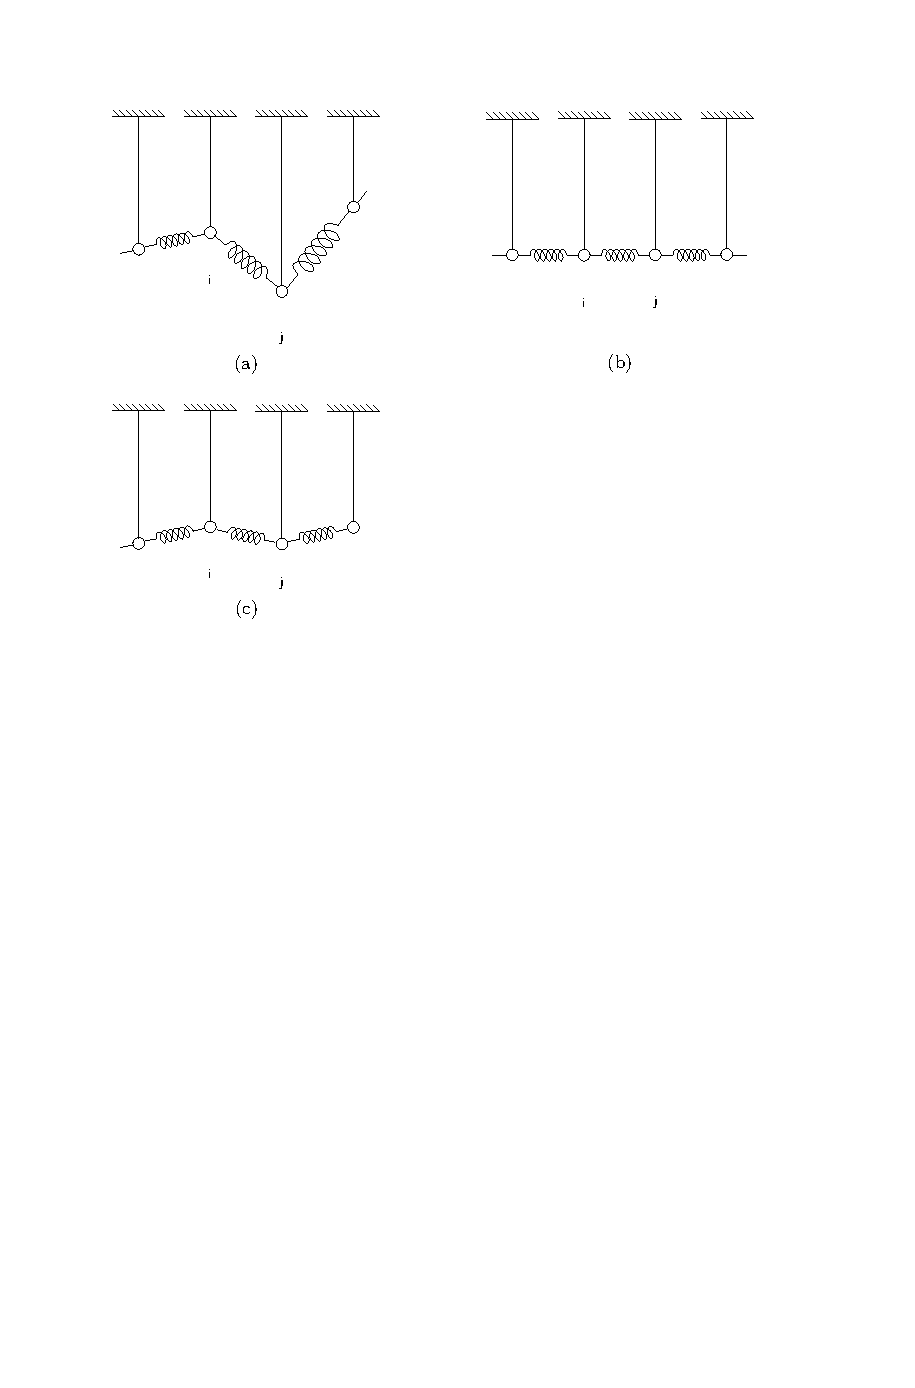
\includegraphics[width=0.70\textwidth]{Economou06fig5-1}
  \caption{
One-dimensional coupled pendulum analog of the tight-binding Hamiltonian,
nearest-neighbor coupling (a). In the periodic case
all pendula and all nearest-neighbor couplings
are identical (b). The double spacing periodic case (c).
(From Economou\rf{Economou06})
  }
  \label{Economou06fig5-1}
\end{figure}
%
\beq
\left(m_i\omega_i^2+\sum_j \kappa_{ij}-m_i\omega^2\right)u_j
- \sum_j \kappa_{ij}u_j=0
\,.
\ee{Economou06(5.13)}
where $u_i$ is the 1-d displacement of the pendulum located at site $i$,
$\omega_i$ is its eigenfrequency in the absence of coupling, and
$\sum_j\kappa_{ij}(u_i-u_j)$ is the force exercised on the pendulum at
the $i$ site as a result of the couplings with all the other pendula;
$m_i$ is the mass at $i$.

If we generalize to 3-d displacements, the problem of coupled pendula is
reduced to that of the ionic (or atomic) motion in solids (by setting
$\omega_i = 0$) since each ion (or atom) is indeed performing small
oscillations around its equilibrium position with the restoring force
being equal to $-\sum_j\kappa_{ij}(u_i-u_j)$. This yields the electronic
eigenfunctions and eigenenergies of the TBM. The eigenmodes are
propagating waves such that the amplitude at each site is the same and
the phase changes in a regular way. For a 2-d square lattice
\beq
E({\bf k}) = \epsilon_0 + 2V[\cos(k_1a)+\cos(k_2a)]
\,,
\ee{Economou06(5.18)}
where $a$ is the lattice constant. In the 1$d$ case, the function
$E({\bf k})$ has an absolute maximum (which corresponds to the upper band
edge) for $k=\pi/a$ or $-\pi/a$ with a value $E_{max}=\epsilon_0+2|V|$;
it has an absolute minimum (which corresponds to a lower band edge) for
$k=0$ with a value $E_{min}=\epsilon_0-2|V|$. Thus the spectrum is a
continuum (a band) extending from $\epsilon_0-2|V|$ to $\epsilon_0+2|V|$.
The bandwidth is $4|V|$.







In his eq.~(5.38) the diagonal
matrix element of the square lattice Greens function is
given by the complete elliptic integral of the first kind\rf{Horiguchi72}
\refeq{Cserti00(38)}.

\bigskip \bigskip

\begin{description}
    \item[2020-10-04 Predrag]
The reason I went above into detail with TBM is (1) it is \catlatt\ for
$s<2$ and (2) has well known elliptic function solutions.
According to
\refeq{Economou06(5.9a)},
the precise formula relating $\epsilon_0$ and $V$ to \catlatt\
stretching factor $s$ is
\[
  s = - \epsilon_0/V
\,,\qquad
u_j \to u_j/\sqrt{-V}
\,.
\]
and the spectrum band extends from $\epsilon_0/|V|-2$ to
$\epsilon_0/|V|+2$, in other words, TBM assumes $|s|<2$.

I assume the band structure for $s<2$ has no counterpart in the hyperbolic,
$s<2$ case, but am not sure.

\PCpost{2018-03-18}{
to Han - can you have a look at the Group Theory course
\HREF{http://birdtracks.eu/courses/PHYS-7143-19/schedule.html\#week8}
{week~8} exercises,
\HREF{http://birdtracks.eu/courses/PHYS-7143-19/soluWeek8Francini.pdf}
{solution~8.3}? I should know this, but I do not, and you have thought
about it: is \catlatt\ in any illuminating sense related to a
tight-binding model? We are not doing QM, but if we formulate the problem
in the continuous space $x\in \reals^d$, rather than the integer lattice
$x\in \integers^d$,  our Hamiltonian is $\delta$ function on each site,
and its neighbors.

If there is a relation, we definitely have to explain that in our paper,
as many colleagues care about couple spin chains and lattices.
}

    \PCpost{2020-01-27}{{\bf to Han -}
For us there is no field $\Xx({z})$ defined over continuum space
$z\in\reals^d$, only $\ssp_z$. Our problems live on the integer lattices
$z\in\integers^d$. This might be called `tight-binding models'. Please
verify whether that's what `tight-binding models' are.
    }

\PCpost{2019-10-10}{Watanabe\rf{Watanabe19}
{\em A proof of the {Bloch} theorem for lattice models}:
``
The Bloch theorem states that the expectation value of the U(1) current
operator averaged over the entire space vanishes for large quantum
systems. The theorem applies as long as all terms in the Hamiltonian are
finite ranged. Finite systems are sensitive to the boundary conditions.
Under the periodic boundary condition, one can only prove that the
current expectation value is inversely proportional to the linear
dimension of the system, while the current expectation value completely
vanishes before taking the thermodynamic limit when the open boundary
condition is imposed. We also provide simple tight-binding models that
clarify the limitation of the theorem in dimensions higher than one.
''
}

    \item[2020-01-13 Predrag]
See also Cserti \etal\rf{Cserti00,CsSzDa11}, in
\refsect{sect:resistors}~{\em Resistor networks}:
The energy-dependent lattice Green's function of the tight-binding
Hamiltonian for a square lattice, his eq.~(30), has energy $E$ playing
the role of our stretching parameter $s$.

\PCpost{2019-07-13}{
Kohler and Cubitt\rf{KohCub19}
{\em Translationally invariant universal classical {Hamiltonians}}
give an explicit construction of a translationally invariant, 2D,
nearest-neighbour, universal classical Hamiltonian with a single free parameter,
drawing on techniques from theoretical computer science, in particular
complexity-theoretic results on tiling problems. Seems too sophisticated for us.
}

  \item[2020-04-19  Predrag]
See also \refchap{chap:chronotope}~{\em Chronotopic literature},
Politi, Torcini and Lepri\rf{PoToLe98}
{\em {Lyapunov} exponents from node-counting arguments}: ``
That resembles the
tight-binding approximation of the lD Schr\"odinger equation (with
imaginary time) in the presence of a random potential, \ie., the Anderson
model.''
\end{description}

\section{Discrete Schr{\"o}dinger equation}
\label{sect:Schrodinger}


\begin{description}
\item[2020-12-06 Predrag]
Marius Lemm, Arka Adhikari and Horng-Tzer Yau, %LeAdYa19
{\em Global eigenvalue distribution of matrices defined by the skew-shift}
\arXiv{1903.11514} study the following question:

\begin{quote}
\emph{Suppose the entries of the large Hermitian matrices $H_N$ are
generated by sampling along the orbits of an ergodic dynamical system. Do
their eigenvalues  still exhibit random matrix statistics, like the
Wigner semicircle law?}
\end{quote}

We will answer this question in the affirmative for the model of $H_N$
defined below, where the underlying dynamical system is generated from
the skew-shift dynamics:
$$
\binom{j}{2} \omega+jy+x \mod 1,
$$
Here $x,y\in \mathbb{T}$ (with $\mathbb{T}$ being the torus) are the
starting positions of the dynamical system and $\omega\in \mathbb{T}$ is
a (typically irrational) parameter called the frequency. The skew-shift
dynamics possesses only weak ergodicity properties, e.g., it is not even
weakly mixing. Nonetheless, it is believed to behave in a quasi-random
way (meaning like an i.i.d.\ sequence of random variables) in various
ways reviewed at the end of the introduction. Moreover, the quasi-random
behavior of the skew-shift should deviate from that of the more rigid
standard shift $j\omega+x\mod 1$ (the circle rotation by an irrational
angle $\omega$). The key difference between the skew-shift and circle
rotation is of course the appearance of a quadratic term $j^2\omega$ for the
skew-shift. This quadratic term has the effect of increasing the
oscillations and thus improving the decay of the exponential sums over
skew-shift orbits. This general fact is a central tenet of analytic
number theory {HL,Mont,W1,W2}, and of our analysis here as well.

{\bf The model.}
Let $\mathbb T$ be the one-dimensional torus, which we identify with
$[0,1]$ in the usual way. For the skew-shift, the role of the ``angle''
is played by the frequency $\omega \in[0,1]$. The skew-shift is then the
transformation
$$
\begin{aligned}
T:&\mathbb{T}^2\to\mathbb{T}^2\\
&(x,y)\mapsto (x+y,y+\omega).
\end{aligned}
$$
We write $T^j$ for the $j$-fold iteration of $T$ and $(T^j(x,y))_1$, for
the first component of the vector $T^j(x,y)\in\mathbb{T}^2$, i.e.,
\beq\label{LeAdYa19:Tjformula}
(T^j(x,y))_1=\binom{j}{2} \omega+jy+x.
\eeq

We consider $2N\times 2N$ Hermitian matrices of the form
$$
H=
\left(\begin{array}{cc} 0&X\\	X^*&0\end{array} \right)
$$
with $X$ an $[N\times N]$ matrix generated from the skew-shift via
\beq\label{LeAdYa19:Xdefn}
X_{i,j}=
\frac{1}{\sqrt{N}}
e\left[\left(\binom{j}{2} \omega_i+jy_i+x_i\right)\right]
\,,\qquad e[t]:=\exp(2\pi i t)
\eeq
Here the $\omega_1,\ldots,\omega_N$ are chosen deterministically (see the
examples below), the $y_1,\ldots,y_N$ in \refeq{LeAdYa19:Xdefn} are sampled
uniformly and independently from $[0,1]$, and the $x_1,\ldots,x_N$ are
arbitrary. (In particular, one can take $x_1=x_2=\ldots=x_N=0$.)

\PCedit{
Predrag: \refeq{LeAdYa19:Xdefn} is an $[N\times N]$ matrix full of
complex phases: it is unlike our 3-banded matrices, I think we can ignore
these papers.
}

Marius Lemm GaTech seminar 2020-04-09: ``
{\em Global eigenvalue distribution of matrices defined by the skew-shift}:
A central question in ergodic theory is whether sequences obtained by
sampling along the orbits of a given dynamical system behave similarly to
sequences of i.i.d. random variables. Here we consider this question from
a spectral-theoretic perspective. Specifically, we study large Hermitian
matrices whose entries are defined by evaluating the exponential function
along orbits of the skew-shift on the 2-torus with irrational frequency.
We prove that their global eigenvalue distribution converges to the
Wigner semicircle law, a hallmark of random matrix statistics, which
evidences the quasi-random nature of the skew-shift dynamics.
''

Kielstra and Lemm  %\rf{KieLem19}
{\em On the finite-size Lyapunov exponent for the Schroedinger operator
with skew-shift potential}
\arXiv{1904.08871}:

A one-dimensional quantum particle living on $\integers$ with energy
$E\in \reals$ is described by the discrete Schr{\"o}dinger equation
\beq\label{LeAdYa19:schr}
\psi_{n+1}+\lambda v_n\psi_n+\psi_{n-1}=E\psi_n,
\eeq
where $\psi=(\psi_n)_{n\in\integers}$ is a sequence in
$\ell^2(\integers;\complex)$. The real-valued potential sequence
$v=(v_n)_{n\in \integers}$ represents the environment that the particle
is subjected to. (The ``coupling constant'' $\lambda>0$ is factored out
for convenience.) Physically, one observes a sudden onset of insulating
behavior in the presence of a random environment (``Anderson
localization''). Mathematically, it is known that for arbitrarily small
$\lambda>0$, the one-dimensional Schr{\"o}dinger operator
\beq\label{LeAdYa19:Hdefn}
(H\psi)_n=\psi_{n+1}+\lambda v_n\psi_n+\psi_{n-1}
\,.
\eeq
has pure point spectrum with exponentially decaying
eigenfunctions\rf{CaKlMa87,KunSou80}.
%\cite{CKM,GMP,KS}.

A natural follow-up question is then: How random does the environment
have to localize the quantum particle? Alternative ``quasi-random''
environments are generated by sampling a nice function along the orbit of
an ergodic dynamical system. This question is interesting from a purely
mathematical ergodic theory perspective, but it also has practical
implications, since computer simulations are mostly based on appropriate
pseudo-random number sequences.

A standing conjecture in this direction concerns the case when the
potential is generated from the nonlinear skew-shift dynamics $T:\mathbb
T^2\to\mathbb T^2$, $T(x,y)=(x+y,y+\omega)$, namely it is of the form
\beq
\label{LeAdYa19:vndefn}
v_n=2\cos\left(\binom{n}{2}\omega +ny+x\right)
\eeq
with $\omega$ irrational (say Diophantine). The key difference between
\refeq{LeAdYa19:vndefn} compared to $v_n=2\cos(n\alpha+\theta)$ is the
appearance of the nonlinear quadratic term $n^2\omega$. The conjecture
states that the associated Schr{\"o}dinger operator $H$ defined by
\refeq{LeAdYa19:Hdefn} is Anderson localized for arbitrarily small
$\lambda>0$ everywhere in the spectrum. Partial results in this vein are
due to
Bourgain %\cite{B}
and
Bourgain-Goldstein-Schlag.  %\cite{BGS}
Note that the conjecture says in particular that the skew-shift dynamics
is appreciably more random-like than the circle rotation where
$v_n=2\cos(n\alpha+\theta)$. (Recall that the latter is only localized
for $\lambda>1$, for us  ${s}>2$.) The observation that the skew-shift is
more quasi-random than the shift has been made in another context by
Rudnick-Sarnak-Zaharescu {RSZ} and others {DR,MY,RS} (concerning the
spacing distribution) and also recently in {ALY} (concerning eigenvalues
of large Hermitian matrices).


\item[2020-12-06 Predrag]
Possibly also of interest:
Marius Lemm and David Sutter
{\em Quantitative lower bounds on the Lyapunov exponent from multivariate
matrix inequalities} \arXiv{2001.09115}:
The Lyapunov exponent characterizes the asymptotic behavior of long
matrix products. Recognizing scenarios where the Lyapunov exponent is
strictly positive is a fundamental challenge that is relevant in many
applications. In this work we establish a novel tool for this task by
deriving a quantitative lower bound on the Lyapunov exponent in terms of
a matrix sum which is efficiently computable in ergodic situations. Our
approach combines two deep results from matrix analysis --- the n-matrix
extension of the Golden-Thompson inequality and the Avalanche-Principle.
We apply these bounds to the Lyapunov exponents of Schrödinger cocycles
with certain ergodic potentials of polymer type and arbitrary correlation
structure. We also derive related quantitative stability results for the
Lyapunov exponent near aligned diagonal matrices and a bound for
almost-commuting matrices.

\item[2020-12-06 Predrag]
Carmona, Klein and Martinelli\rf{CaKlMa87} {\em Anderson localization for
Bernoulli and other singular potentials}:

Bernoulli potentials are potentials that take only two values
\[
\mu  = p\delta(v-a)+ (1-p)\delta(v-b)
\,,\qquad
0<p<1
\,.
\]

Kunz and Souillard\rf{KunSou80} {\em Sur le spectre des op{\'e}rateurs
aux diff{\'e}rences finies al{\'e}atoires} is presumably similar -
models for Anderson localization, we do not need them here.


\end{description}

\section{Harper's model}
\label{sect:Harper}

\begin{description}
\item[2020-12-06 Predrag]
Kielstra and Lemm  %\rf{KieLem19}
{\em On the finite-size Lyapunov exponent for the Schroedinger operator
with skew-shift potential}
\arXiv{1904.08871} write: ``
For example, one can consider
$v_n=2\cos(n\alpha+\theta)$ generated from sampling cosine along an
irrational circle rotation; this is the Harper\rf{Harper55}  or
almost-Mathieu\rf{Simon82} model. It turns out that these linear underlying
dynamics only produce localization for sufficiently strong potentials,
namely only for $\lambda>1$ (for us, ${s}>2$)\rf{Jitomirskaya99}. %{Jit}.
''

%{Jit}
Jitomirskaya\rf{Jitomirskaya99}
{\em Metal-insulator transition for the almost Mathieu operator}.

Svetlana Jitomirskaya, Lyuben Konstantinov and Igor Krasovsky
% \rf{JiKoKr20}
\\
{\em On the spectrum of critical almost Mathieu operators in the rational case}
\\
\arXiv{2007.01005}:

The Harper operator, a.k.a. the discrete magnetic Laplacian
%  name ``discrete magnetic Laplacian'' was first introduced by
%  M. Shubin in \cite{shu}.}, is
a tight-binding model of an electron confined to a 2D square lattice in a
uniform magnetic field orthogonal to the lattice plane and with flux
$2\pi\alpha$ through an elementary cell. It acts on
$\ell^2(\integers^2)$ and
is usually given in the Landau gauge representation
\begin{equation} \label{JiKoKr20(1)} %{alpha}
(H(\alpha)\psi)_{m,n}=\psi_{m,n-1}+\psi_{m,n+1}+e^{-i2\pi\alpha
  n}\psi_{m-1,n}+e^{i2\pi\alpha n}\psi_{m+1,n},
\end{equation}
first considered by Peierls\rf{Peierls33},
who noticed that it makes the
Hamiltonian separable and turns it into the direct integral in $\theta$
of operators on $\ell^2(\mathbb{Z})$ given by:
\begin{equation}
(H_{\alpha, \theta}\,\field)_n  =
   \field_{n-1} + 2\cos2\pi(\alpha n+\theta)\,\field_{n} + \field_{n+1}
\,, \qquad \alpha, \theta \in [0, 1).
\ee{JiKoKr20(2)}
In physics literature, it also appears under the names Harper's or  the
Azbel-Hofstadter model, with both names  used also for the discrete
magnetic Laplacian $H(\alpha)$.  In mathematics, it is universally called
the critical almost Mathieu operator\rf{Simon82}.
% This name was originally introduced by Barry Simon \cite{flu}.
In addition to importance in
physics, this model is of special interest, being at the boundary of two
reasonably well understood regimes: (almost) localization and (almost)
reducibility, and not being amenable to methods of either side.

%{shu}           M.A. Shubin. Discrete Magnetic Laplacian,
%  Commun. Math. Phys. {\bf 164}, 259–275 (1994)

Simon\rf{Simon82}
{\em Almost periodic Schr{\'o}dinger operators: {A review}}\\
{[...]} one-dimensional Schrödinger equation,
$H = -d^2/dx^2 + V(x)$ with $V(x)$
almost periodic and the discrete (= tight binding) analog, i.e., the
doubly infinite Jacobi matrix
\beq
h_{ij} = \delta_{i,j+1}  + V_i\delta_{i,j} + \delta_{i,j-1}
\ee{Simon82}
with $V_n$ almost periodic on the integers.

% {\bf Remark} {\it
% Equations \eqref{Chambersodd} and \eqref{Chamberseven} are variants of
% the well-known Chambers' relation for $H_{\frac{p_0}{q_0}, \theta}$
% \cite{Chambers65} (see \cite{BellissardSimon82} for a proof):

The \emph{Chambers' formula} presents the dependence of the
determinant of the almost Mathieu operator with $\alpha={p}/\cl{}$
restricted to the period $\cl{}$ with Floquet boundary conditions, on
the phase $\theta$ and quasimomentum $k$. In the critical case it is
given by
% (see, e.g., \cite{Last94})
\beq
\det(\jMorb_{\theta, k,\cl{}} - E) =
\Delta(E) -2 (-1)^{\cl{}}(\cos(2 \pi \cl{} \theta) + \cos(k \cl{})),
\ee{JiKoKr20(7)} %{ChambersFormula}
where $\ell \in \mathbb{Z}/\cl{}$, and in our notation
\refeq{JiKoKr20(2)} is written as
\refeq{eq:CatMapNewton5}
\beq
\ssp_{\ell+1}  -  {s}_\ell\, \ssp_{\ell} + \ssp_{\ell-1}
    =
-\Ssym{\ell}
\,,
\ee{Harper}
with site-dependent stretching ${s}_\ell$ (so not a Toeplitz matrix,
compare with \refeq{shiftMatrix}, \refeq{HLdDJacobian},
\refeq{errorVecsTrevers},\refeq{PV2configJ},\refeq{eq:orbitJPVtempJ},
\refeq{catalattLxTrop})
\beq
\jMorb_{\theta, k,\cl{}} :=
\begin{pmatrix}
-{s}_{0} & 1 & 0 & 0 & \cdots & 0 & 0 & e^{-i k \cl{}} \\
1 & -{s}_{1} & 1 & 0 & \cdots & 0 & 0 & 0 \\
0 & 1 & -{s}_{2} & 1 & \cdots & 0 & 0 & 0 \\
\vdots & \vdots & \vdots & \vdots & \ddots & \vdots & \vdots & \vdots \\
0 & 0 & 0 & 0 & \cdots & 1 & -{s}_{\cl{}-2} & 1 \\
e^{i k \cl{}} & 0 & 0 & 0 & \cdots & 0 & 1 & -{s}_{\cl{}-1}
\end{pmatrix}\,,
\ee{JiKoKr20(8)}
compare with the {\jacobianOrb} $\jMorb$ \refeq{jMorbInfin}.
For Harper model, stretching ${s}_\ell$ is given by
\beq
{s}_\ell(\theta) = -2 \cos(2\pi\frac{p}{\cl{}}\ell + \theta)
        \,,\qquad
{s}(x)           = x)
\,,
\ee{JiKoKr20(9)}
and the discriminant $\Delta$
% \footnote{In \cite{Last94}, the discriminant differs from $\Delta(E)$
% by the factor $(-1)^{q_0}$.},
is independent of $\theta$ and $k$.
They obtain a formula of this type for
$\det(B_{\theta, k,\ell} - E).$

\item[2020-12-06 Predrag]
For $\alpha\in\integers$ this is a Helmholtz problem with
stretching parameter ${s}=2\cos 2\pi(\theta)$.

For rational $\alpha$ has periodic ${s}$\rf{Hofstadter76},
as in \refeq{JiKoKr20(9)}.
Note the relative-periodic corner phases $e^{\pm i k q}$
in \refeq{JiKoKr20(8)}).

Hofstadter\rf{Hofstadter76}
{\em Energy levels and wave functions of {Bloch} electrons in rational
and irrational magnetic fields} writes about rational case: ``
Algebra reveals the fact that this condition on $\alpha$ is precisely
that of rationality: We now proceed, making full use of this somewhat
bizarre ansatz.
''

He, as everybody else, sooner or later, rewrites \refeq{Harper} in
the ``\PV\'' `two-configuration representation'\rf{PerViv}
matrix $\jMps$
%=\MatrixII{0}{1}
%          {-1}{s}
\refeq{PerViv:2confRepMat},
\beq
 \left(\begin{array}{c}
 \Delta\field_{\zeit}  \\
 \Delta\field_{\zeit+1}
 \end{array} \right )=
 \left(\begin{array}{cc}
  0 & 1       \\
 -1 & {s}_{\zeit}
 \end{array} \right )
 \left(\begin{array}{c}
 \Delta\field_{\zeit-1}  \\
 \Delta\field_{\zeit}
 \end{array} \right ) %\mbox{ mod } 1
\,.
\ee{CL18:StateSpCatMap}
(note `upside-down' 2D vector), and concerns himself with
the rational,
energy $\tr \jMps^m<2$, oscillatory case.

Note, it's only about the order of recurrence, nobody says the systems
should be Hamiltonian / Lagrangian, works for dissipative systems as
well.

The famed butterfly is a plot
of the eigenvalues for all rational phases $\alpha$.

\item[2020-12-06 Predrag]
        \PCedit{
I am looking at \refeq{JiKoKr20(2)} because this is a different way to
introduce a nonlinearity than the H\'enon CML \refeq{PolTor92(2.1)}
because for irrational $\alpha$
it has a quadratic dependence on the lattice site,
\[
2\cos(2\pi\alpha n) = 2- (2\pi\alpha n)^2 +\cdots
\,.
\]
        }
Nevertheless, this discrete Schr{\"o}dinger is very different from
\templatt, so one more Sunday has been wasted (?) on learning other stuff.

\item[2021-06-25 Indubala Satija]
{\em Geometry, Number Theory and the Butterfly Spectrum of Two-Dimensional
  Bloch Electrons}
\arXiv{2106.1387}:

We take a deeper dive into the geometry and the number theory that underlay
the butterfly graphs of the Harper and the generalized Harper models of Bloch
electrons in a magnetic field. Root of the number theoretical characteristics
of the fractal spectrum is traced to a close relationship between the Farey
tree -- the hierarchical tree that generates all rationals and the Wannier
diagram -- a graph that labels all the gaps of the butterfly graph. The
resulting Farey-Wannier hierarchical lattice of trapezoids provides
geometrical representation of the nested pattern of butterflies in the
butterfly graph. Some features of the energy spectrum such as absence of some
of the Wannier trajectories in the butterfly graph fall outside the number
theoretical framework, can be stated as a simple rule of "minimal violation
of mirror symmetry". In a generalized Harper model, Farey-Wannier
representation prevails as the lattice regroups to form some hexagonal unit
cells creating new {\it species} of butterflies.


\end{description}

\section{Frenkel-Kontorova model}
\label{sect:FrenkelKontorova}

\begin{description}

    \PCpost{2021-02-01}{
The \eqva\ and \reqva\ of Frenkel-Kontorova models\rf{AuAb90}, widely studied in
literature, might be closely related to \henlatt\ and $\phi^4$ lattices.

It is difficult stuff, safely ignored, for now:)

Note the text below
\refeq{MacMei83(17)}
and
\refeq{MraRin12:RR}.

Search for
\textbf{2019-12-12} \emph{Meisinger and Ogilvie} notes in this blog.
    }

\item[2021-02-01 Anna Vainchtein] (U. Pittsburgh)

\emph{Traveling waves in a driven Frenkel-Kontorova lattice}:
Variants of Frenkel-Kontorova model, originally proposed to describe
dislocations in crystal lattices, have been widely used to study a
variety of physical phenomena, including dynamics of twin boundaries and
domain walls, crystal growth, charge-density waves, Josephson junctions
and DNA denaturation. I discuss properties and stability of traveling
waves in chains of Frenkel-Kontorova type driven by a constant external
force. After reviewing some earlier studies for piecewise-smooth variants
of the model, where exact and semi-analytical solutions can be
constructed, I will describe numerical results for a fully nonlinear
damped driven chain from a recent work with J. Cuevas-Maraver (U. of
Sevilla), P.  Kevrekidis (U. of Mass.) and H. Xu (Huazhong U.). In this
setting, \PCedit{traveling wave solutions are computed as fixed points of
a nonlinear map}. [...] Exploring the spectral stability of the obtained
waveforms, we identify, at the level of numerical accuracy of our
computations, a precise criterion for instability of the traveling wave
solutions: monotonically decreasing portions of the kinetic curve always
bear an unstable eigendirection.

The recorded talk will be available
\HREF{https://sites.google.com/view/nwcswebinar/speakers} {here}.
It is a difficult subject, but our case - \eqva\ and \reqva\ is perhaps a
trivial case described in this literature.

\item[2019-06-26 Predrag]
Mramor and Rink\rf{MraRin12}
{\em Ghost circles in lattice {Aubry-Mather} theory}, \arXiv{1111.5963}:

``Monotone lattice recurrence relations such as the Frenkel-Kontorova
lattice, arise in Hamiltonian lattice mechanics as models for
ferromagnetism and as discretization of elliptic PDEs.
They are a multidimensional counterpart of monotone twist maps.''

The paper has an appendix of twist maps, refers to Mather and
Forni\rf{MatFor94} {\em Action minimizing orbits in {Hamiltomian}
systems}. Example of exact symplectic twist maps are the Chirikov
standard map and convex billiards. I think the focus in all this work is
on {\em integrable}, not chaotic:
``Under generic conditions, the Poincar\'e return map of a $2$ degree of
freedom Hamiltonian system near an elliptic equilibrium point is an exact
symplectic twist map. In this case, the corresponding twist map is close
to {\it integrable}, so that it allows for the application of various
kinds of perturbation theory\rf{MatFor94}.''
Lectures on {\em Equidistribution of periodic orbits: An overview of
classical VS quantum results} by Degli Esposti, Graffi, and Isola in {\em
Transition to Chaos in Classical and Quantum Mechanics}\rf{Graffi94} are
also of interest.

Twist maps often admit a variational structure, so that the solutions
$x:\integers^d\to \reals$ are the stationary points of a formal action
function $W(x)$. Given any rotation vector $\omega\in \reals^d$,
Aubry-Mather theory establishes the existence of a large collection of
solutions of $\nabla W(x)=0$ of rotation vector $\omega$. For irrational
$\omega$, this is the {\em Aubry-Mather set}. It consists of global
minimizers and it may have gaps.

The part relevant to our \catlatt\ is the idea of studying globally
stationary solutions by means of a formal gradient. We do not really know
how to find all \twots\ in 2 or more dimensions, even though we know how
to count them, right?
They study the parabolic gradient flow
$\frac{dx}{dt} = -\nabla W(x)$
and prove that every Aubry-Mather set can be
interpolated by a continuous gradient-flow invariant family, the
so-called `ghost circle'. The existence of these ghost circles is known
in dimension $d=1$, for rational rotation vectors and Morse action
functions.

\medskip
{\bf $d$-dimensional Frenkel-Kontorova lattice:}
Here, the goal is to find a
$d$-dimensional ``lattice configuration'' $x:\integers^d\to \reals$ that satisfies
\begin{align}\label{MraRin12:RR}
V'(x_i) - (\Delta x)_i = 0 \  \ \mbox{for all} \ i\in \mathbb{Z}^d
\,.
\end{align}
The smooth function $V: \mathbb{R} \to \mathbb{R}$
satisfies $V(\xi+1)=V(\xi)$ for all $\xi\in\reals$. It has the interpretation
of a periodic onsite potential.

I like their definition of the discrete Laplace operator
$\Delta:\mathbb{R}^{\mathbb{Z}^d}\to\mathbb{R}^{\mathbb{Z}^d}$, defined as
\begin{align}\label{Lap}
(\Delta x)_i := \frac{1}{2d} \sum_{||j-i||=1} \!\! (x_j - x_i)
\ \mbox{for all} \ i \in \integers^d
\,.
\end{align}
where $||i||:=\sum_{k=1}^{d}|i_k|$.
Thus, $(\Delta x)_i$ is the average of the quantity $x_j-x_i$ computed
over the lattice points that are nearest to that with index $i$, \ie, the
graph Laplacian\rf{Pollicott01,Cimasoni12} \refeq{gaphLapl} for the case
of hypercubic lattice, or the ``central difference operator''\rf{PerViv}.

One can think of (\ref{MraRin12:RR}) as a naive discretization of the
nonlinear elliptic partial differential equation $V'(u) - \Delta u=0$ for
a function $u: \mathbb{R}^d\to \mathbb{R}$ and $x_i = u(i)$.

Eq.~(\ref{MraRin12:RR}) is relevant for statistical mechanics, because it is
related to the Frenkel-Kontorova Hamiltonian lattice differential
equation
\begin{align} \label{FKHam}
\frac{d^2 x_i}{dt^2} + V'(x_i) - (\Delta x)_i = 0 \ \mbox{for all} \ i\in\mathbb{Z}^d.
\end{align}
This differential equation describes the motion of particles under the
competing influence of an onsite periodic potential field and nearest
neighbor attraction. Eq.~(\ref{MraRin12:RR}) describes its
stationary solutions.

In dimension $d=1$, the solutions of equation (\ref{MraRin12:RR})
correspond to orbits of the Chirikov standard map
$T_V:\mathbb{A}\to\mathbb{A}$ of the annulus.

The Frenkel-Kontorova problem (\ref{MraRin12:RR}) is an example from a quite
general class of lattice recurrence relations to which the results of
this paper apply. These are recurrence relations for which there exists,
for every $j\in \integers^d$, a real-valued ``local potential'' function
$S_j:\reals^{\integers^d}\to \reals$ so that the relation can be written in the form
\begin{align}\label{RRR1}
\sum_{j\in \integers^d} \partial_iS_j(x) = 0\ \mbox{for all} \ i\in \mathbb{Z}^d .
\end{align}
It turns out that for the Frenkel-Kontorova problem (\ref{MraRin12:RR}), such
local potentials exist and it is easy to check that they are given by
 \begin{align}\label{FKpotential}
 S_j(x):= V(x_j) + \frac{1}{8d} \sum_{||k-j||=1}(x_k-x_j)^2.
 \end{align}
For the general problem (\ref{RRR1}), the functions $S_j(x)$ will be
required to satisfy some rather restrictive hypotheses.
% that will be explained in detail in Section \ref{problemsetup}.
Physically, the most
important of these hypotheses is the {\it monotonicity} condition. It is
a discrete analogue of ellipticity for a PDE. Among the more technical
hypotheses is one that guarantees that the sums in expression
(\ref{RRR1}) are finite. For the purpose of this introduction, it
probably suffices to say that the potentials (\ref{FKpotential}) of
Frenkel-Kontorova are prototypical for the $S_j(x)$ that we have in mind.

\indent
It is important to observe that the solutions of (\ref{RRR1}) are
precisely the stationary points of the formal sum
\begin{align}\label{potentialW}
W(x):=\sum_{j\in\integers^d} S_j(x).
\end{align}
This follows because differentiation of (\ref{potentialW}) with respect
to $x_i$ produces exactly equation (\ref{RRR1}) and it explains why
solutions to (\ref{RRR1}) are sometimes called {\it stationary}
configurations.
%and for every finite subset $B\subset \integers^d$ the ``finite action function''
 %\begin{align}\label{finiteaction}
%W_B(x) := \sum_{j\in B} S_j(x) \ .
%\end{align}
%A short computation shows that when $i\in \mathring{B}:= \{i\in B\ | \ ||j-i||=1\Rightarrow  j\in B \}$, then $\frac{dW_B(x)}{dx_i}= V'(x_i) - (\Delta x)_i$. Thus, a solution $x:\integers^d\to\reals$ of (\ref{MraRin12:RR}) is characterized by the property that for every finite subset $B\subset \mathbb{Z}^d$ and every configuration $y$ with support in $\mathring{B}$, it holds that
%$$\left. \frac{d}{d\varepsilon} \right|_{\varepsilon = 0} W_B(x+\varepsilon y) = 0 \ . $$

\noindent
In the case that the periodic onsite potential $V(\xi)$ vanishes, the
Frenkel-Kontorova equation (\ref{MraRin12:RR}) reduces to the discrete Laplace
equation $\Delta x= 0$, for which it is easy to point out solutions. For
instance, when $\xi\in \mathbb{R}$ is an arbitrary number and $\omega \in
\mathbb{R}^d$ is an arbitrary vector, then the linear functions
$x^{\omega, \xi}: \mathbb{Z}^d\to\mathbb{R}$ defined by
$$x_i^{\omega, \xi} :=\xi + \langle \omega, i\rangle $$
%= \xi + \sum_{k=1}^d \omega_k \! \cdot \! i_k \ $$
obviously satisfy $\Delta x = 0$. It moreover turns out that the
$x^{\omega, \xi}$ are {\it action-minimizers}, in the sense that for
every finite subset $B\subset \integers^d$ and every $y:\integers^d\to \reals$ with support
in $B$, it holds that
\[
\sum_{j\in \integers^d} \left( S_j(x^{\omega,\xi}+ y)
                        - S_j(x^{\omega, \xi}) \right) \geq 0 \,.
\]
Note that this sum is actually finite and can be interpreted as
$W(x^{\omega, \xi}+y)-W(x^{\omega,\xi})$.
\begin{definition}
Let $x:\mathbb{Z}^d\to\mathbb{R}$ be a $d$-dimensional configuration.
We say that $\omega\in \mathbb{R}^d$ is the {\it rotation vector} of $x$
if for all $i\in \mathbb{Z}^d$, the limit
\[
\lim_{n\to \infty} \frac{x_{ni}}{n} \ \mbox{exists and is equal to} \ \langle \omega, i\rangle
\,.
\]
\end{definition}
\noindent
Clearly, the rotation vector of $x^{\omega, \xi}$ is equal to $\omega$.
On the other hand, in dimension $d\neq 1$, a solution to (\ref{MraRin12:RR}) does
not necessarily have a rotation vector. An example is the hyperbolic
configuration $x^h$ defined by $x^h_i=i_1 i_2\cdots i_{d-1} i_d$ which
solves $\Delta x =0$.
\end{description}

\section{Mean field theory for the Ising model}
\label{sect:MFT-Ising}
%NKHM15.tex
%arxiv.org/abs/1502.04074
%Eur. Phys. J. B (2017) 90: 7
%DOI: 	10.1140/epjb/e2016-70641-1

According to E. Br{\'e}zin and J. Zinn-Justin,
finite-size mean field theory for the Ising model
% Finite size effects in phase transitions
% https://doi.org/10.1016/0550-3213(85)90379-7
is described by the distribution
\beq
p_{\rm MFT}(m)\,\propto\,\exp\left(-Nf(m)\right),
\ee{NKHM15cw}
where $N$ is the number of spins and the free energy (the large-deviation
potential) at reduced temperature $\tilde{t}$ is
\beq
f(m)\,=\,\frac{1}{2} \tilde{t}\,m^2+\frac{1}{4!} m^4,
\ee{NKHM15fe}
to leading order in $N$.


\section{Clock model}
\label{sect:clock}

The \HREF{https://en.wikipedia.org/wiki/Potts_model\#Free_field_solution}
{free field solutions} of Potts models are most directly related to our
dynamical considerations. If all states are allowed the underlying set of
states is given by a full shift. If neighboring spins are only allowed in
certain specific configurations, then the state space is given by a
subshift of finite type. The partition function may then be written as a
trace of the adjacency matrix, specifying which neighboring spin values
are allowed.

The \HREF{https://en.wikipedia.org/wiki/Z_N_model} {wiki} says:
The \emph{$Z_N$ model}, a generalization of the Ising model, sometimes
known as the \emph{clock model} or the \emph{vector Potts model}, is
defined by assigning a spin value at each node $r$ on a graph, with the
spins taking values $S_r=\exp{\frac{2\pi i q}{N}}$, where $q\in
\{0,1,\ldots,N-1\}$. The spins therefore take values in the form of
complex roots of unity. The spin assigned to each node of the $Z_N$ model
is pointing in any one of $N$ directions. The Boltzmann weights for a
general edge $rr'$ are:
\[
w\left(r,r'\right)
=\sum_{k=0}^{N-1}x_{k}^{\left(rr'\right)}\left(S_{r}S_{r'}^*\right)^k
\]
where $*$ denotes complex conjugation and the $x_{k}^{\left(rr'\right)}$
are related to the interaction strength along the edge $rr'$. Note that
$x_{k}^{\left(rr'\right)}=x_{N-k}^{\left(rr'\right)}$ and $x_0$ is often
set to 1. The (real valued) Boltzmann weights are invariant under the
transformations $S_r \rightarrow \omega^k S_r$ and $S_r \rightarrow
S^{*}_{r}$, the universal rotation and the reflection respectively.

\begin{quote}
The $q$-state clock model discretizes the rotor angle $[0,2\pi]$, so that
is not what we need; \catlatt\ has discrete winding numbers. It is $X-Y$
model that has our $\Ssym{n}$ as vortex charges, and interactions between
$(\mbox{mod}\;1)$ angles, except those are no the nearest neighbor, but
logarithmic.
\end{quote}

The local magnetic moment or ``spin'', a 2D vector dimensionless vector
of magnitude one, $S_i=(\cos( 2\pi q k), \sin( 2\pi q k))$, where
$k=0,1,\cdots,q-1$, at site $i$ can point in any of the $q$ directions in
a given plane, with equal probability for all $q$ values. The isotropic
Hamiltonian for such a system can be written as:
\beq
H = - \frac{J}{2} \sum_{\left< ij \right>} S_i\cdot S_j
-B\cdot\sum_{i}S_i
\,,
\ee{NVPSV18eq:h}

In the \emph{$q$-state clock model}  on each lattice point there is a vector
spin pointing to $q$ different directions, which differ by the angle
$2\pi/q$.
% clipped from \arXiv{1307.5512}
The 2D $q$-state clock model is defined by the Hamiltonian
\beq
H = - J \sum_{\left< ij \right>} \cos(\theta_i - \theta_j)
-h\sum_{i}\cos {\theta}_{i}
\,,
\ee{BMMK13eq:h}
where $J$ is interaction strength, the summation is over the nearest
neighbors, $h$ is the applied weak magnetic field in units of $J/\mu$,
where $\mu$ is the magnetic moment of each spin usually set to 1, and
$\theta_i=2\pi{n_i}/q$ with $n_i=0,\ldots,q-1$.
Generalized Eq.~(\ref{BMMK13eq:h}) is of form
\[
H =  \sum_{\left< ij \right>} V(\theta_i - \theta_j)
   -h\sum _{i}\cos {\theta }_{i}
\,,
\]
where the spin-interaction potential $V$ has the $Z_q$ symmetry.
The Villain $q$-state clock model has
\[
V(\phi) = -\frac{J}{\beta} \ln \left\{ \sum_{n=-\infty}^{\infty}
\exp\left[ -\beta (\phi - 2\pi n)^2/2 \right] \right\}
\,,
\]
where  $\beta \equiv 1/(k_B T)$ with the Boltzmann constant $k_B$ and
temperature $T$. This potential has been introduced to separate the
vortex degrees of freedom from the spin-wave degrees of freedom as an
approximate version of the $XY$ model. %~\cite{savit}.
The Villain clock model on the square lattice possesses
self-duality. %~\cite{savit}.
%\bibitem [{\citenamefont {Savit}(1980)}]{savit}%
%  \BibitemOpen
%  \bibfield  {author} {\bibinfo {author} {\bibfnamefont {R.}~\bibnamefont
%  {Savit}},\ }\href@noop {} {\bibfield  {journal} {\bibinfo  {journal} {Rev.
%  Mod. Phys.}\ }\textbf {\bibinfo {volume} {52}},\ \bibinfo {pages} {453}
%  (\bibinfo {year} {1980})}\BibitemShut {NoStop}%

The case q=2 corresponds to the Ising model, the case q=3 is a special
case of the Potts model. Already for q=4 the phase diagram is more
complicated that for the Ising model: there are 3 phases, instead of 2.


Once the partition function is known, the thermodynamic observables, such
as internal energy U, specific heat C, and entropy S, can be calculated
by employing\rf{NVPSV18}:
\beq
U(T) = T^2 \frac{\partial~}{\partial T} \ln Z(T,B)
\,.
\ee{NVPSV18intEn}
\beq
C(T) =
\frac{\partial U}{\partial T}
\,,
\ee{NVPSV18specHeat}
\beq
S(T) = \frac{U}{T} + \ln Z(T, B)
\,.
\ee{NVPSV18entropy}
The lattice average of the spin configuration, equivalent to the
magnetization per site M, is given by
\beq
M =  \frac{1}{N}\sum_{j}S_j
\,.
\ee{NVPSV18magn}
They go on to compute the internal energy U and the specific heat C.

In all of the literature the focus is on  Berezinskii-Kosterlitz-Thouless
(BKT) transition,  between a topological  phase  and  the
high-temperature  paramagnetic (or disordered) phase, and phases possible
for $q>5$. If there is no continuous symmetry,  existence of standard
ferromagnetic order is allowed at low but finite temperature.

We are focused on the high-temperature  paramagnetic (or disordered)
phase.

\begin{description}
    \PCpost{2019-12-12} {                       \toSect{sect:FrenkelKontorova}
Meisinger and Ogilvie %\rf{MeiOgl13}
{\em The Sign Problem, PT Symmetry and Abelian Lattice Duality}
\arXiv{1306.1495}:
For Abelian models in the class of {lattice field theories with the
fundamental fields which are elements $z= \exp(i\theta)$ of Z(N) or U(1),
with complex actions}, lattice duality maps models with complex actions
into dual models with real actions.

Explicit duality relations are given for models for spin and gauge models
based on Z(N) and U(1) symmetry groups. The dual forms are
generalizations of the Z(N) chiral clock model and the lattice
Frenkel-Kontorova model, respectively.

We begin with duality for $d=2$ $Z(N)$ models with a chemical potential
% using the methods of \cite{Elitzur:1979uv}
for the Villain, or heat kernel, action. Defining the site-based spin
variables as $\exp\left(2\pi im(x)/N\right)$, with $m(x)$ an integer
between $0$ and $N$, the partition function is given by
\beq
Z[J,\mu\delta_{\nu,2}]
=\sum_{m}\sum_{n_{\nu}}\exp\left[-\frac{J}{2}\sum_{x,\nu}\left(\frac{2\pi}{N}\partial_{\nu}m\left(x\right)-i\mu\delta_{\nu2}-2\pi n_{\nu}\left(x\right)\right)^{2}\right]
\ee{MeiOgl13}
where $\partial_{\nu}m(x)\equiv m(x+\hat{\nu})-m(x)$ and the sum
over link variables $n_{\nu}(x)\in Z$ ensures periodicity. Using
the properties of the Villain action, we can write
\bea
Z[J,\mu\delta_{\nu,2}]
    &=&
\left(2\pi J\right)^{-dV/2}\sum_{m}\sum_{p_{\nu}}\exp\left[-\frac{1}{2J}\sum_{x,\nu}p_{\nu}^{2}\left(x\right)
    \right.
    \ceq
    \left.\quad\quad
+\,i\sum_{x,\nu}p_{\nu}\left(x\right)\left(\frac{2\pi}{N}\partial_{\nu}m\left(x\right)-i\mu\delta_{\nu2}\right)
  \right]
  \nnu
\eea
where $V$ is the number of sites on the lattice such that $dV$ is
the number of links. Summation over the $m\left(x\right)$'s give
a set of delta function constraints:
\[
Z[J,\mu\delta_{\nu,2}]
=\left(2\pi J\right)^{-dV/2}\sum_{p_{\nu}}\exp\left[-\frac{1}{2J}\sum_{x,\nu}p_{\nu}^{2}\left(x\right)+\sum_{x,\nu}p_{2}\left(x\right)\mu\right]\prod_{x}\delta_{\partial\cdot p,0\left(N\right)}
\]
where the notation in the Kronecker delta function indicates $\partial\cdot p=0$
modulo $N$. We introduce a dual bond variable $\tilde{p}_{\rho}\left(X\right)$
associated with the dual lattice via $p_{\nu}\left(x\right)=\epsilon_{\nu\rho}\tilde{p}_{\rho}\left(X\right)$
and note that the constraint on $p_{\nu}$ is solved by $\tilde{p}_{\rho}\left(X\right)=\partial_{\rho}\tilde{q}\left(X\right)+N\tilde{r}_{\nu}\left(X\right)$.
We have
\bea
Z[J,\mu\delta_{\nu,2}]
    &=&
\left(2\pi J\right)^{-dV/2}\sum_{\tilde{q}}\sum_{\tilde{r}_{\nu}}\exp\left[-\frac{1}{2J}\sum_{x,\nu}\left(\partial_{\rho}\tilde{q}\left(X\right)+N\tilde{r}_{\nu}\left(X\right)\right)^{2}
    \right.
    \ceq
    \left.\quad\quad
+\mu\sum_{x,\nu}\left(\partial_{1}\tilde{q}\left(X\right)+N\tilde{r}_{1}\left(X\right)\right)\right]
\nnu
\eea
which leads to
\[
Z[J,\mu\delta_{\nu,2}]=\left(2\pi J\right)^{-dV/2}\exp\left[+\frac{V}{2}J\mu^{2}\right]Z[\frac{N^{2}}{4\pi^{2}J},-i\frac{2\pi J\mu}{N}\delta_{\nu,1}]
\]
 The generalized duality here is
\begin{eqnarray}
J & \rightarrow & \tilde{J}=\frac{N^{2}}{4\pi^{2}J}\\
\mu\delta_{\nu,2} & \rightarrow & \tilde{\mu}\delta_{\nu,1}=-i\frac{2\pi J\mu}{N}\delta_{\nu,1}.
\end{eqnarray}
The dual of the original model, which has a complex action, is a chiral
$Z(N)$ model with a real action.
    }

    \PCpost{2019-12-12} {
Jing Chen, Hai-Jun Liao, Hai-Dong Xie, Xing-Jie Han, Rui-Zhen Huang, Song
Cheng, Zhong-Chao Wei, Zhi-Yuan Xie, and Tao Xiang,
{\em Phase transition of the q-state clock model: duality and tensor
renormalization}, \arXiv{1706.03455}.

Now, memorize the authors:)
    }

    \PCpost{2019-12-22} {

    }

    \PCpost{2019-12-22} {

    }

\end{description}

\section{$X$-$Y$ model}
\label{sect:XY}

\begin{description}

    \PCpost{2019-12-22} {
Peter N. Meisinger and Michael C. Ogilvie, %\rf{MeiOgl13}
{\em The Sign Problem, PT Symmetry and Abelian Lattice Duality},
\arXiv{1306.1495}\\
(see also Meisinger and Ogilvie {\em The sign problem and Abelian lattice
duality}, \arXiv{1311.5515}):
The partition function of the two-dimensional XY model with an imaginary
chemical potential term has the form
\[
Z[K,\mu\delta_{\nu,2}]=\int_{S^{1}}\left[d\theta\right]\sum_{n_{\nu}}\exp\left[-\frac{K}{2}\sum_{x,\nu}\left(\partial_{\nu}\theta\left(x\right)-i\mu\delta_{\nu2}-2\pi n_{\nu}\left(x\right)\right)^{2}\right].
\]
Using the properties of the Villain action, we have
\[
Z[K,\mu\delta_{\nu,2}]=\int_{S^{1}}\left[d\theta\right]\prod_{x,\nu}\sum_{p_{\nu}\left(x\right)\in Z}\frac{1}{\sqrt{2\pi K}}e^{-p_{\nu}^{2}\left(x\right)/2K}e^{ip_{\nu}\left(x\right)\left(\nabla_{\nu}\theta\left(x\right)-i\delta_{\nu2}\mu\right)}.
\]
[...]
The partition function is now
\[
Z=\sum_{\{m\left(X\right)\}\in Z}\frac{1}{\sqrt{2\pi K}}e^{-\sum_{X}\left[\sum_{\nu}\left(\nabla_{\nu}m\left(X\right)\right)^{2}/2K+\mu\nabla_{1}m\left(X\right)\right]}.
\]
The final step is to introduce a new field $\phi(x)\in R$ using a
periodic $\delta$-function, effectively performing a Poisson resummation:
\[
Z=\int_{R}\left[d\phi\left(X\right)\right]e^{-\sum_{X}\left[\sum_{\nu}\left(\nabla_{\nu}\phi\left(X\right)\right)^{2}/2K+\mu\nabla_{1}\phi\left(X\right)\right]}\sum_{\{m\left(X\right)\}\in Z}e^{2\pi im\left(X\right)\phi\left(X\right)}.
\]
If we keep only the $m=1$ contributions, we have a lattice sine-Gordon
model
\[
Z=\int_{R}\left[d\phi\left(X\right)\right]\exp\left[-\sum_{X,\mu}\frac{1}{2K}\left(\nabla_{\mu}\phi\left(X\right)\right)^{2}-\sum_{X}\mu\nabla_{1}\phi\left(X\right)+\sum_{X}2y\cos\left(2\pi\phi\left(X\right)\right)\right]
\]
with $y=1$. This will be recognized as a two-dimensional lattice
version of the Frenkel-Kontorova model, a sine-Gordon model with an
additional term proportional to $\mu$. For each fixed value of $X_{2}$,
the term $\sum_{X}\nabla_{1}\phi\left(X\right)$ counts the number
of kinks on that slice: The particles in the original representation
manifest as lattice kinks in the dual representation.

        } % end \PCpost{2019-12-22}

    \PCpost{2020-06-15} {
I do not even know what this is:
Mazel, Stuhl and Suhov,
{\em High-density hard-core model on $\integers^2$
and norm equations in ring $\integers [{\sqrt[6]{-1}}]$},\\
\arXiv{1909.11648}. They study the Gibbs statistics of high-density
hard-core configurations on a unit square lattice $\integers^2$, for a
general Euclidean exclusion distance $D$, with $D^2=a^2+b^2$,
$a,b\in\integers$. Pictorially, the problem is to study properties of
configurations formed by non-overlapping `hard spheres' of a given
diameter (or exclusion distance) $D$ with specified positions of the
centers.

They  say that a configuration $\phi$ is periodic if there exist two
linearly independent vectors $e_1$, $e_2$ such that $\phi (x)=\phi
(x+e_1)=\phi (x+e_2)$. If a periodic configuration $\phi$ contains the
origin, we say that $\phi$ is a {\it sub-lattice}. The parallelogram with
vertices $0$, $e_1$, $e_2$, $e_1+e_2$ is a {\it fundamental
parallelogram} (FP) for $\phi$. We always assume that $e_{1,2}$ are
chosen so that the shorter diagonal of the FP divides it into two
triangles with non-obtuse angles; one of these triangles, with a vertex
at the origin, is referred to as a {\it fundamental triangle} (FT). They
say that a sub-lattice is isosceles or non-isosceles if the FT is
isosceles or not.

The term $\integers^2$-triangle means a triangle with vertices in $\integers^2$.
Without loss of generality we will assume that one of the vertices is at
the origin $(0,0)$.

They say that a given value $D$ exhibits \ {\it sliding} \ if exist  two
or more M-triangles ${\tt T}^{(1)}$, ${\tt T}^{(2)}$, $\ldots$, with (i)
a common side called a {\it sliding base}, with two common vertices, and
(ii) distinct third vertices lying in the same half-plane relative to the
shared side.
Sliding leads to a multitude of periodic and non-periodic ground states
characterized by layered or staggered patterns. The point is that under
sliding there are countably many periodic and continuum of non-periodic
ground states.
    }
\end{description}
